% Options for packages loaded elsewhere
\PassOptionsToPackage{unicode}{hyperref}
\PassOptionsToPackage{hyphens}{url}
\PassOptionsToPackage{dvipsnames,svgnames,x11names}{xcolor}
%
\documentclass[
  super,
  preprint,
  3p]{elsarticle}

\usepackage{amsmath,amssymb}
\usepackage{iftex}
\ifPDFTeX
  \usepackage[T1]{fontenc}
  \usepackage[utf8]{inputenc}
  \usepackage{textcomp} % provide euro and other symbols
\else % if luatex or xetex
  \usepackage{unicode-math}
  \defaultfontfeatures{Scale=MatchLowercase}
  \defaultfontfeatures[\rmfamily]{Ligatures=TeX,Scale=1}
\fi
\usepackage{lmodern}
\ifPDFTeX\else  
    % xetex/luatex font selection
\fi
% Use upquote if available, for straight quotes in verbatim environments
\IfFileExists{upquote.sty}{\usepackage{upquote}}{}
\IfFileExists{microtype.sty}{% use microtype if available
  \usepackage[]{microtype}
  \UseMicrotypeSet[protrusion]{basicmath} % disable protrusion for tt fonts
}{}
\makeatletter
\@ifundefined{KOMAClassName}{% if non-KOMA class
  \IfFileExists{parskip.sty}{%
    \usepackage{parskip}
  }{% else
    \setlength{\parindent}{0pt}
    \setlength{\parskip}{6pt plus 2pt minus 1pt}}
}{% if KOMA class
  \KOMAoptions{parskip=half}}
\makeatother
\usepackage{xcolor}
\setlength{\emergencystretch}{3em} % prevent overfull lines
\setcounter{secnumdepth}{5}
% Make \paragraph and \subparagraph free-standing
\ifx\paragraph\undefined\else
  \let\oldparagraph\paragraph
  \renewcommand{\paragraph}[1]{\oldparagraph{#1}\mbox{}}
\fi
\ifx\subparagraph\undefined\else
  \let\oldsubparagraph\subparagraph
  \renewcommand{\subparagraph}[1]{\oldsubparagraph{#1}\mbox{}}
\fi

\usepackage{color}
\usepackage{fancyvrb}
\newcommand{\VerbBar}{|}
\newcommand{\VERB}{\Verb[commandchars=\\\{\}]}
\DefineVerbatimEnvironment{Highlighting}{Verbatim}{commandchars=\\\{\}}
% Add ',fontsize=\small' for more characters per line
\usepackage{framed}
\definecolor{shadecolor}{RGB}{241,243,245}
\newenvironment{Shaded}{\begin{snugshade}}{\end{snugshade}}
\newcommand{\AlertTok}[1]{\textcolor[rgb]{0.68,0.00,0.00}{#1}}
\newcommand{\AnnotationTok}[1]{\textcolor[rgb]{0.37,0.37,0.37}{#1}}
\newcommand{\AttributeTok}[1]{\textcolor[rgb]{0.40,0.45,0.13}{#1}}
\newcommand{\BaseNTok}[1]{\textcolor[rgb]{0.68,0.00,0.00}{#1}}
\newcommand{\BuiltInTok}[1]{\textcolor[rgb]{0.00,0.23,0.31}{#1}}
\newcommand{\CharTok}[1]{\textcolor[rgb]{0.13,0.47,0.30}{#1}}
\newcommand{\CommentTok}[1]{\textcolor[rgb]{0.37,0.37,0.37}{#1}}
\newcommand{\CommentVarTok}[1]{\textcolor[rgb]{0.37,0.37,0.37}{\textit{#1}}}
\newcommand{\ConstantTok}[1]{\textcolor[rgb]{0.56,0.35,0.01}{#1}}
\newcommand{\ControlFlowTok}[1]{\textcolor[rgb]{0.00,0.23,0.31}{#1}}
\newcommand{\DataTypeTok}[1]{\textcolor[rgb]{0.68,0.00,0.00}{#1}}
\newcommand{\DecValTok}[1]{\textcolor[rgb]{0.68,0.00,0.00}{#1}}
\newcommand{\DocumentationTok}[1]{\textcolor[rgb]{0.37,0.37,0.37}{\textit{#1}}}
\newcommand{\ErrorTok}[1]{\textcolor[rgb]{0.68,0.00,0.00}{#1}}
\newcommand{\ExtensionTok}[1]{\textcolor[rgb]{0.00,0.23,0.31}{#1}}
\newcommand{\FloatTok}[1]{\textcolor[rgb]{0.68,0.00,0.00}{#1}}
\newcommand{\FunctionTok}[1]{\textcolor[rgb]{0.28,0.35,0.67}{#1}}
\newcommand{\ImportTok}[1]{\textcolor[rgb]{0.00,0.46,0.62}{#1}}
\newcommand{\InformationTok}[1]{\textcolor[rgb]{0.37,0.37,0.37}{#1}}
\newcommand{\KeywordTok}[1]{\textcolor[rgb]{0.00,0.23,0.31}{#1}}
\newcommand{\NormalTok}[1]{\textcolor[rgb]{0.00,0.23,0.31}{#1}}
\newcommand{\OperatorTok}[1]{\textcolor[rgb]{0.37,0.37,0.37}{#1}}
\newcommand{\OtherTok}[1]{\textcolor[rgb]{0.00,0.23,0.31}{#1}}
\newcommand{\PreprocessorTok}[1]{\textcolor[rgb]{0.68,0.00,0.00}{#1}}
\newcommand{\RegionMarkerTok}[1]{\textcolor[rgb]{0.00,0.23,0.31}{#1}}
\newcommand{\SpecialCharTok}[1]{\textcolor[rgb]{0.37,0.37,0.37}{#1}}
\newcommand{\SpecialStringTok}[1]{\textcolor[rgb]{0.13,0.47,0.30}{#1}}
\newcommand{\StringTok}[1]{\textcolor[rgb]{0.13,0.47,0.30}{#1}}
\newcommand{\VariableTok}[1]{\textcolor[rgb]{0.07,0.07,0.07}{#1}}
\newcommand{\VerbatimStringTok}[1]{\textcolor[rgb]{0.13,0.47,0.30}{#1}}
\newcommand{\WarningTok}[1]{\textcolor[rgb]{0.37,0.37,0.37}{\textit{#1}}}

\providecommand{\tightlist}{%
  \setlength{\itemsep}{0pt}\setlength{\parskip}{0pt}}\usepackage{longtable,booktabs,array}
\usepackage{calc} % for calculating minipage widths
% Correct order of tables after \paragraph or \subparagraph
\usepackage{etoolbox}
\makeatletter
\patchcmd\longtable{\par}{\if@noskipsec\mbox{}\fi\par}{}{}
\makeatother
% Allow footnotes in longtable head/foot
\IfFileExists{footnotehyper.sty}{\usepackage{footnotehyper}}{\usepackage{footnote}}
\makesavenoteenv{longtable}
\usepackage{graphicx}
\makeatletter
\def\maxwidth{\ifdim\Gin@nat@width>\linewidth\linewidth\else\Gin@nat@width\fi}
\def\maxheight{\ifdim\Gin@nat@height>\textheight\textheight\else\Gin@nat@height\fi}
\makeatother
% Scale images if necessary, so that they will not overflow the page
% margins by default, and it is still possible to overwrite the defaults
% using explicit options in \includegraphics[width, height, ...]{}
\setkeys{Gin}{width=\maxwidth,height=\maxheight,keepaspectratio}
% Set default figure placement to htbp
\makeatletter
\def\fps@figure{htbp}
\makeatother

\makeatletter
\makeatother
\makeatletter
\makeatother
\makeatletter
\@ifpackageloaded{caption}{}{\usepackage{caption}}
\AtBeginDocument{%
\ifdefined\contentsname
  \renewcommand*\contentsname{Table of contents}
\else
  \newcommand\contentsname{Table of contents}
\fi
\ifdefined\listfigurename
  \renewcommand*\listfigurename{List of Figures}
\else
  \newcommand\listfigurename{List of Figures}
\fi
\ifdefined\listtablename
  \renewcommand*\listtablename{List of Tables}
\else
  \newcommand\listtablename{List of Tables}
\fi
\ifdefined\figurename
  \renewcommand*\figurename{Figure}
\else
  \newcommand\figurename{Figure}
\fi
\ifdefined\tablename
  \renewcommand*\tablename{Table}
\else
  \newcommand\tablename{Table}
\fi
}
\@ifpackageloaded{float}{}{\usepackage{float}}
\floatstyle{ruled}
\@ifundefined{c@chapter}{\newfloat{codelisting}{h}{lop}}{\newfloat{codelisting}{h}{lop}[chapter]}
\floatname{codelisting}{Listing}
\newcommand*\listoflistings{\listof{codelisting}{List of Listings}}
\makeatother
\makeatletter
\@ifpackageloaded{caption}{}{\usepackage{caption}}
\@ifpackageloaded{subcaption}{}{\usepackage{subcaption}}
\makeatother
\makeatletter
\@ifpackageloaded{tcolorbox}{}{\usepackage[skins,breakable]{tcolorbox}}
\makeatother
\makeatletter
\@ifundefined{shadecolor}{\definecolor{shadecolor}{rgb}{.97, .97, .97}}
\makeatother
\makeatletter
\makeatother
\makeatletter
\makeatother
\journal{Journal Name}
\ifLuaTeX
  \usepackage{selnolig}  % disable illegal ligatures
\fi
\usepackage[]{natbib}
\bibliographystyle{elsarticle-num}
\IfFileExists{bookmark.sty}{\usepackage{bookmark}}{\usepackage{hyperref}}
\IfFileExists{xurl.sty}{\usepackage{xurl}}{} % add URL line breaks if available
\urlstyle{same} % disable monospaced font for URLs
\hypersetup{
  pdftitle={Fundamental Problems with the Evidence Base for Adolescent Depression Treatments.},
  pdfauthor={Argyris Stringaris; Charlotte Burman; Dayna Bhudia; Carmen Moreno; Samuele Cortese; Georgina Krebs},
  pdfkeywords={depression, adolescents, antidepressants, psychotherapy},
  colorlinks=true,
  linkcolor={blue},
  filecolor={Maroon},
  citecolor={Blue},
  urlcolor={Blue},
  pdfcreator={LaTeX via pandoc}}

\setlength{\parindent}{6pt}
\begin{document}

\begin{frontmatter}
\title{Fundamental Problems with the Evidence Base for Adolescent
Depression Treatments. \\\large{A conceptual and quantiative
re-appraisal.} }
\author[1]{Argyris Stringaris%
\corref{cor1}%
}
 \ead{a.stringaris@ucl.ac.uk} 
\author[1]{Charlotte Burman%
%
}
 \ead{c.burman@ucl.ac.uk} 
\author[1]{Dayna Bhudia%
%
}
 \ead{d.bhudia@ucl.ac.uk} 
\author[2]{Carmen Moreno%
%
}
 \ead{cmoreno@hggm.es} 
\author[3]{Samuele Cortese%
%
}
 \ead{samuele.cortese@soton.ac.uk} 
\author[1]{Georgina Krebs%
%
}
 \ead{g.krebs@ucl.ac.uk} 

\affiliation[1]{organization={University College London, Divisions of
Psychiatry and Psychology and Language Science},addressline={1-19
Torrington Place},city={London, UK},country={United
Kingdom},countrysep={,},postcode={WC1E 7HB},postcodesep={}}
\affiliation[2]{organization={Hospital Gregorio Marañón, Department of
Psychiatry},addressline={46 C. del
Dr.~Esquerdo},city={Madrid},country={Spain},countrysep={,},postcode={28007},postcodesep={}}
\affiliation[3]{organization={University of Southampton, Centre for
Innovation in Mental Health (CIMH), School of
Psychology},addressline={Highfield Campus, Building
44},city={Southampton},country={United
Kingdom},countrysep={,},postcode={SO17 1BJ},postcodesep={}}

\cortext[cor1]{Corresponding author}






        
\begin{abstract}
To follow
\end{abstract}





\begin{keyword}
    depression \sep adolescents \sep antidepressants \sep 
    psychotherapy
\end{keyword}
\end{frontmatter}
    \ifdefined\Shaded\renewenvironment{Shaded}{\begin{tcolorbox}[sharp corners, boxrule=0pt, interior hidden, frame hidden, borderline west={3pt}{0pt}{shadecolor}, breakable, enhanced]}{\end{tcolorbox}}\fi

\hypertarget{introduction}{%
\section{Introduction}\label{introduction}}

Depression is the leading cause of disability in adolescents and
influential guidelines recommend that it be treated with either
psychotherapy or anti-depressant medication or their combination. The
evidence base for this recommendation typically derives from the
appraisal of randomised controlled trials (RCTs) in which one modality
(psychotherapy or anti-depressants) are compared against a control
condition. In this paper we identify a series of fundamental problems
with this appraisal and make recommendations on how it can be improved.

Guidelines make implicit and explicit \ldots{} comparisons\ldots{}

Network metanalyses\ldots{}

Jureidini approach\ldots summarises.

This state of affairs is reflected in textbooks and also in what
trainees in psychiatry and psychology learn QUOTE.

Yet, is this approach correct?

This approach relies on a (explicit or more often implicit) comparison
of the two treatment modalities. Ideally, a comparison between the
treatment modalities should be direct, that is head to head. Only one
such trial exists in adolescent depression (from the TADS study, see
below) which showed that fluoxetine was superior to both cognitive and
behavioural therapy (CBT) as well as placebo, and that CBT did not
differentiate from placebo. Apart from this one study, all other
comparisons indirect, that is, they have to be inferred from comparing
studies where an antidepressant or a psychotherapy is compared to a
control condition; the control conditions for antidepressant studies is
the placebo (standard also in the rest of medicine), whilst controls for
psychotherapy studies can vary substantially from waiting list, to
treatment as usual to an attention control, such as psychoeducation.
These comparisons therefore have to rely on testing whether the
following simple equality holds or not,

\begin{equation}\protect\hypertarget{eq-1}{}{Effect_{Med} = Effect_{Psy}}\label{eq-1}\end{equation}

where \emph{Effect} denotes the effect on depression that either
medication (\emph{Med} ) or psychotherapy (\emph{Psy}) have. This
comparison is achieved by comparing some measure of effect,
e.g.~percentage response or standardised mean difference, for each
medication and psychotherapy. The simplest way of doing such a
comparison is to take pooled estimates of such effects from metanalyses
of each anti-depressants and psychotherapy and compare them informally.
A more formal way of doing this is through a network metanalysis, which
uses any direct comparisons to infer indirect ones.

Yet for the indirect comparison to be valid, several assumptions need to
hold. The most important of these assumptions can be summarised using
the technical term \emph{ceteris paribus}, meaning that the results of
this comparison are valid if all else is equal. Two important such
assumptions are: a) that the control conditions for each antidepressant
and psychotherapy trials are equal---we call this the \emph{equality of
controls} assumption. b) that the effects of each treatment modality
have been derived from the same underlying population, that is that the
people who have received the treatment are similar on important
parameters on average--this we call the \emph{one population}
assumption.

Starting with the \emph{equality of controls}, its importance can be
easily intuited by expanding equation 1 to include the comparisons on
which each side of that equation rests:

\begin{equation}\protect\hypertarget{eq-2}{}{Effect_{MedActive} - Effect_{MedControls} = Effect_{PsyActive} - Effect_{PsyControls}}\label{eq-2}\end{equation}

where MedActive and PsyActive are the active arms of antidepressant and
psychotherapy trials, respectively, and MedControls and PsyControls the
respective control arms. The assumption here has to be that the controls
are equal, that is, \[ Effect_{MedControls} = Effect_{PsyControls}\]. A
few simple examples help illustrate why this assumption is important Let
the two modalities of treatment be medication and surgery, and let there
be a trial for each modality. In the medication trial 80\% of
participants respond to the antihypertensive and only 40\% to placebo;
in the surgery trial, 40\% of people respond to surgery and 0\% to sham.
If one relied on Equation 1 to compare the treatments they would arrive
at the absurd conclusion that the two treatments are equal and recommend
to a patient that it does not really matter which one they choose.
Playing around with numbers in which no equality of the respective
control arms is required, leads to other risible conclusions.

Yet, surprisingly, a focus on the equality of controls is largely absent
from appraisals of the evidence of medication and psychotherapy.

Moving on to the \emph{one population} assumption, this can be
formalised

\citet{stringarisDevelopmentalPathwaysChildhood2014}

\hypertarget{figures-and-tables}{%
\section{Figures and tables}\label{figures-and-tables}}

\begin{figure}

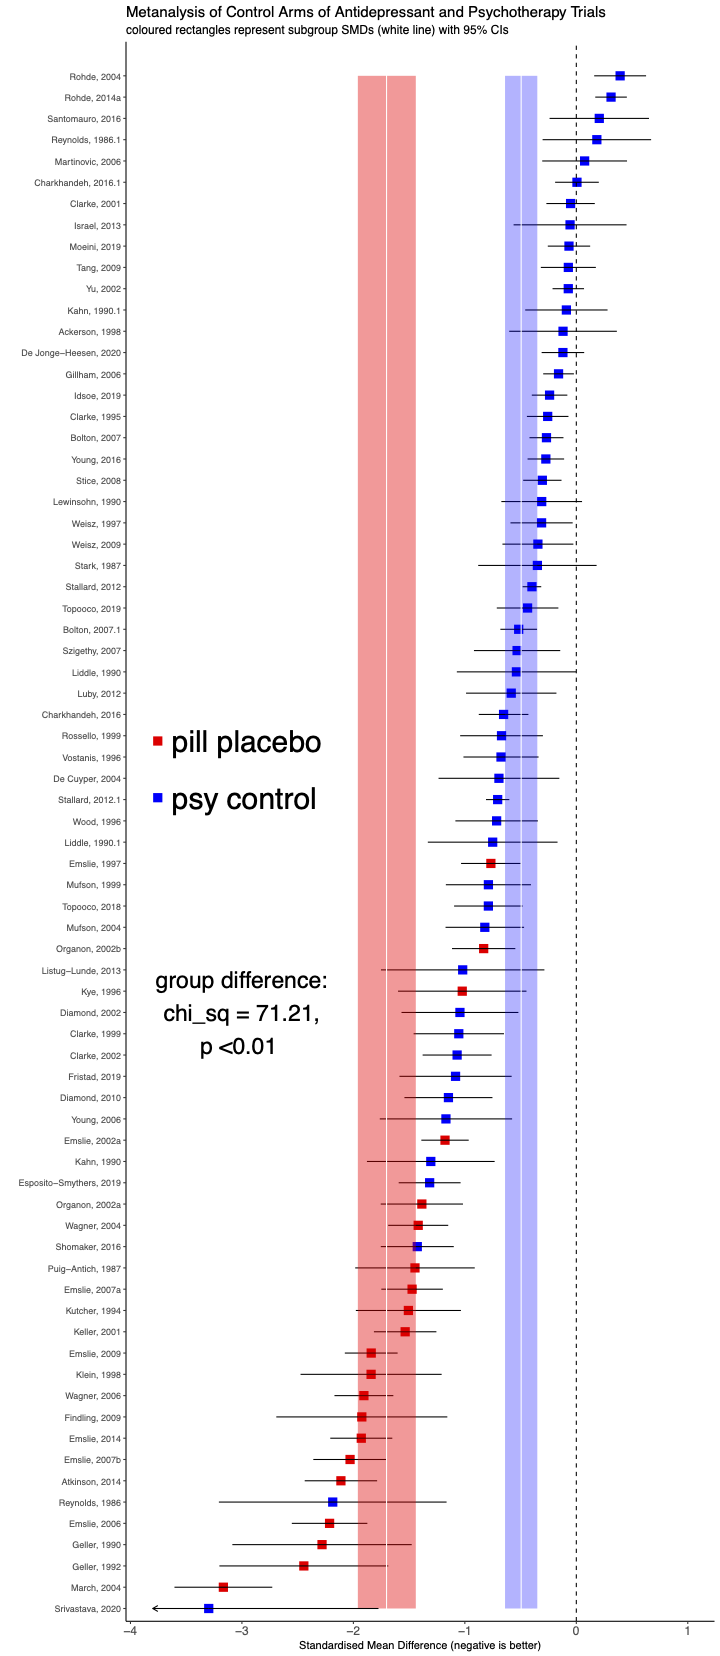
\includegraphics[width=12.5in,height=\textheight]{forestplot.png} \hfill{}

\caption{Forest Plot of Control Arms by the Control Arm of Each
Treatment Modality.}

\end{figure}

\begin{verbatim}
\end{verbatim}

\hypertarget{tables-coming-from-rtable}{%
\section{Tables coming from RTable}\label{tables-coming-from-rtable}}

\begin{Shaded}
\begin{Highlighting}[]
\NormalTok{knitr}\SpecialCharTok{::}\FunctionTok{kable}\NormalTok{(}\FunctionTok{head}\NormalTok{(mtcars)[,}\DecValTok{1}\SpecialCharTok{:}\DecValTok{4}\NormalTok{])}
\end{Highlighting}
\end{Shaded}

\hypertarget{tbl-simple}{}
\begin{longtable}[]{@{}lrrrr@{}}
\caption{\label{tbl-simple}Caption centered above table}\tabularnewline
\toprule\noalign{}
& mpg & cyl & disp & hp \\
\midrule\noalign{}
\endfirsthead
\toprule\noalign{}
& mpg & cyl & disp & hp \\
\midrule\noalign{}
\endhead
\bottomrule\noalign{}
\endlastfoot
Mazda RX4 & 21.0 & 6 & 160 & 110 \\
Mazda RX4 Wag & 21.0 & 6 & 160 & 110 \\
Datsun 710 & 22.8 & 4 & 108 & 93 \\
Hornet 4 Drive & 21.4 & 6 & 258 & 110 \\
Hornet Sportabout & 18.7 & 8 & 360 & 175 \\
Valiant & 18.1 & 6 & 225 & 105 \\
\end{longtable}


  \bibliography{emotion\_concepts\_paper.bib}


\end{document}
